%\documentclass[11pt]{book}
%\usepackage{palatino}
%\usepackage{amsfonts,amsmath,amssymb}
%% \usepackage{graphicx}
%
%
%\ifx\pdftexversion\undefined
%    \usepackage[dvips]{graphicx}
%\else
%    \usepackage[pdftex]{graphicx}
%    \usepackage{epstopdf}
%    \epstopdfsetup{suffix=}
%\fi
%
%\usepackage{color}
%
%\begin{document}
%
%%%%%%%%%%%%%%%%%%%%%%%%%%%%%%%%%%%%%%%%%
%% Problem Set 5
%%%%%%%%%%%%%%%%%%%%%%%%%%%%%%%%%%%%%%%%%
%
%\pagestyle{empty}
%{\noindent\bf Spring 2023 \hfill Brandon~Parmanand}
%\vskip 16pt
%\centerline{\bf University of Central Florida}
%\centerline{\bf College of Business}
%\vskip 16pt
%\centerline{\bf QMB 6911}
%\centerline{\bf Capstone Project in Business Analytics}
%\vskip 10pt
%\centerline{\bf Solutions:  Problem Set \#5}
%\vskip 32pt
%\noindent
%
%
%
%
%\section{Histogram and Density of Log. {\color{red} Fly Reel} Prices}
%
%To begin visually analyzing the data, 
%include plots of the density that were created from last milestones.
%
%\subsection{All Houses Together}
%
%Start with the log of prices because prices were skewed.
%Figure \ref{fig:hist_dens_log_price} is
%a histogram of the logarithm of house prices, 
%along with a rug plot and a kernel density estimate. 
%%
%\begin{figure}[h!]
%  \centering
%  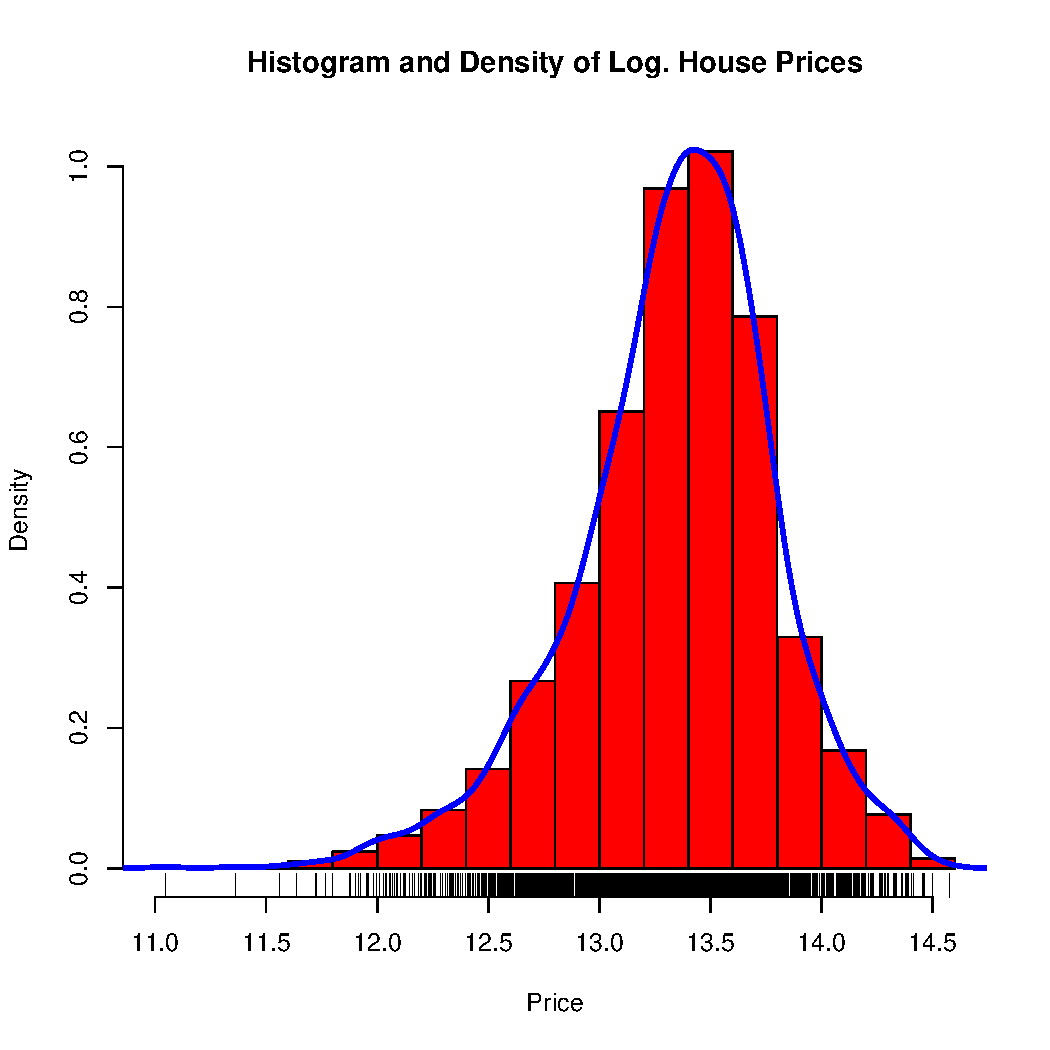
\includegraphics[scale = 0.5, keepaspectratio=true]{../Figures/hist_dens_log_price}
%  \caption{Relative Histogram of Fly Reel Prices} \label{fig:hist_dens_log_price}
%\end{figure}
%% 
%After taking logs, we can see that the distribution is
%approximately symmetric, now with a slight skew to the left. 
% 
%
%
%\clearpage
%\pagebreak
%\subsection{Comparison By Type of Buyer}
%
%Now we investigate the prices of houses that are owner occupied 
%compared to rental homes.
%Figure \ref{fig:dens_by_TypeOfBuyer} shows the 
%kernel density estimate of the prices of 
%owner occupied houses in blue
%and rental houses in red.
%% 
%I observed more variability in the prices of rental houses. 
%Owner-occupied houses are in the higher price range compared to rentals.
%
%{\color{red} As I mentioned earlier, the default bandwidth makes this very smooth, 
%so that the distributions look artificially normal or mixed normal.
%Also, this feature could be applied to other variables for more insight.}
%
%
%
%\begin{figure}[h!]
%  \centering
%  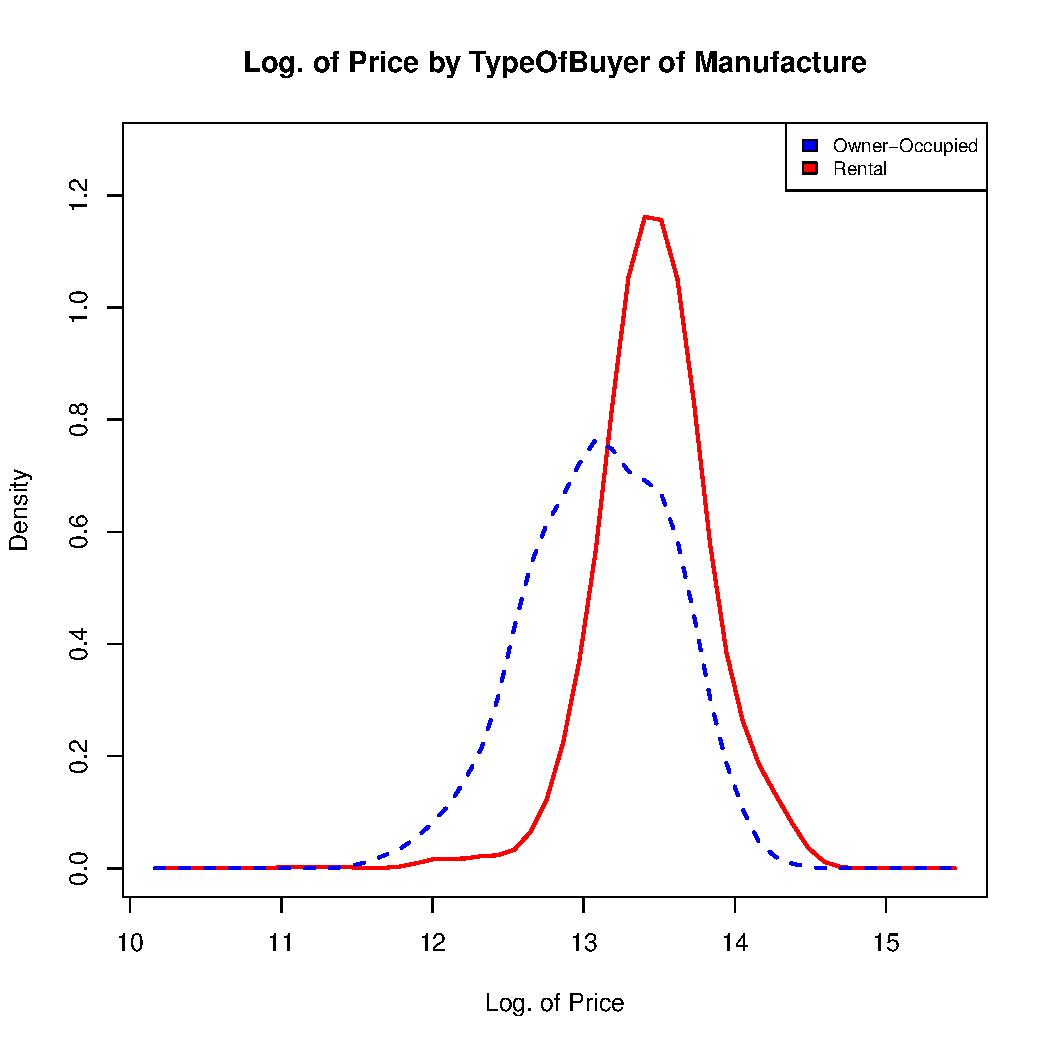
\includegraphics[scale = 0.5, keepaspectratio=true]{../Figures/dens_by_TypeOfBuyer}
%  \caption{Densities of Log.House Prices by Country of Manufacture} \label{fig:dens_by_TypeOfBuyer}
%\end{figure}
%
%
%\clearpage
%\pagebreak

I observed more variability in the prices of rental houses. 
Owner-occupied houses are in the higher price range compared to rentals.

\section*{Scatterplot Matrices}


\subsection*{Scatterplots of Numeric Variables}

Figure \ref{fig:slpom_num_only} depicts a matrix of scatterplots
of the numeric variables in the dataset.


\begin{figure}[h!]
  \centering
  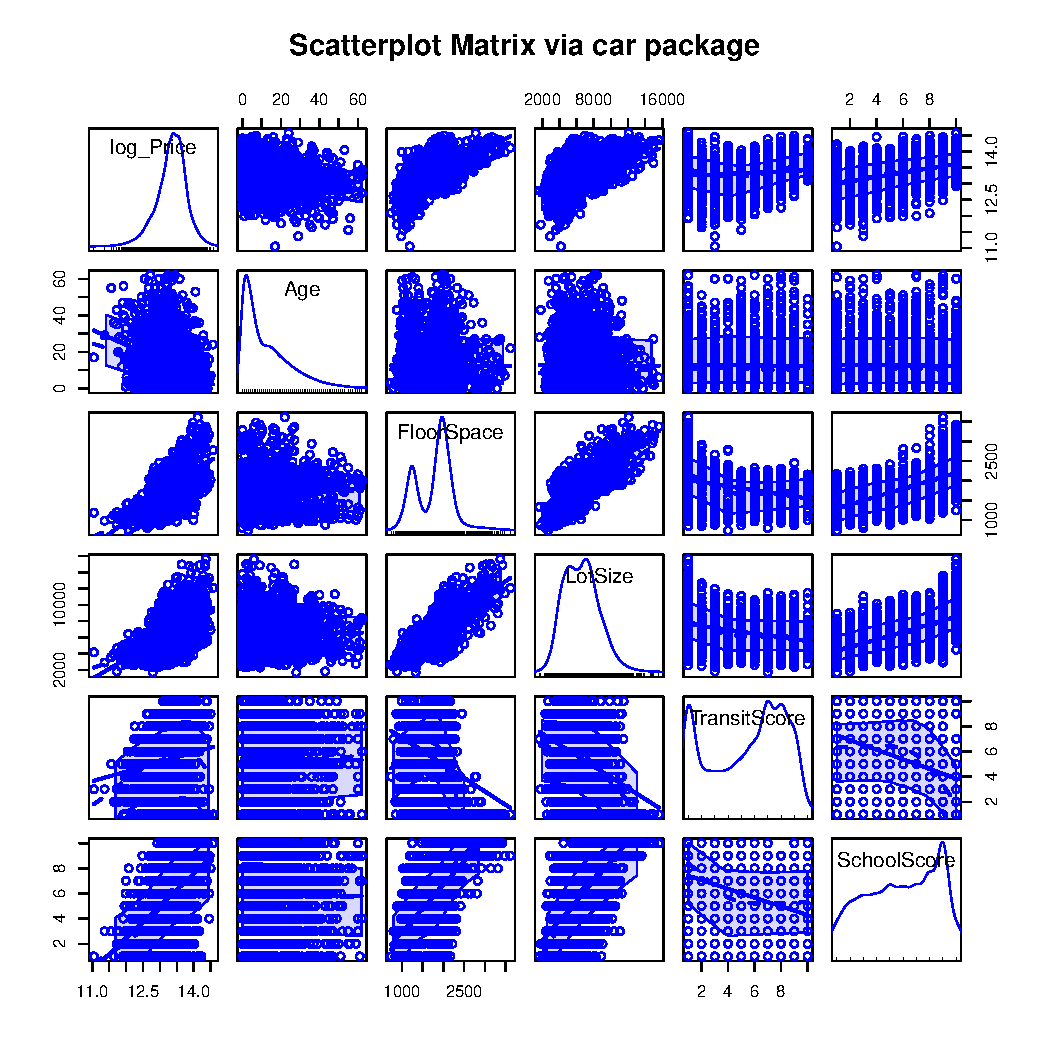
\includegraphics[scale = 0.5, keepaspectratio=true]{../Figures/slpom_num_only}
  \caption{Scatterplots of Numeric Variables} \label{fig:slpom_num_only}
\end{figure}


\pagebreak
\subsection*{Scatterplots with Categorical Variables}

Figure \ref{fig:slpom_by_buyer} depicts a matrix of scatterplots
of some categorical variables in the dataset.

\begin{figure}[h!]
  \centering
  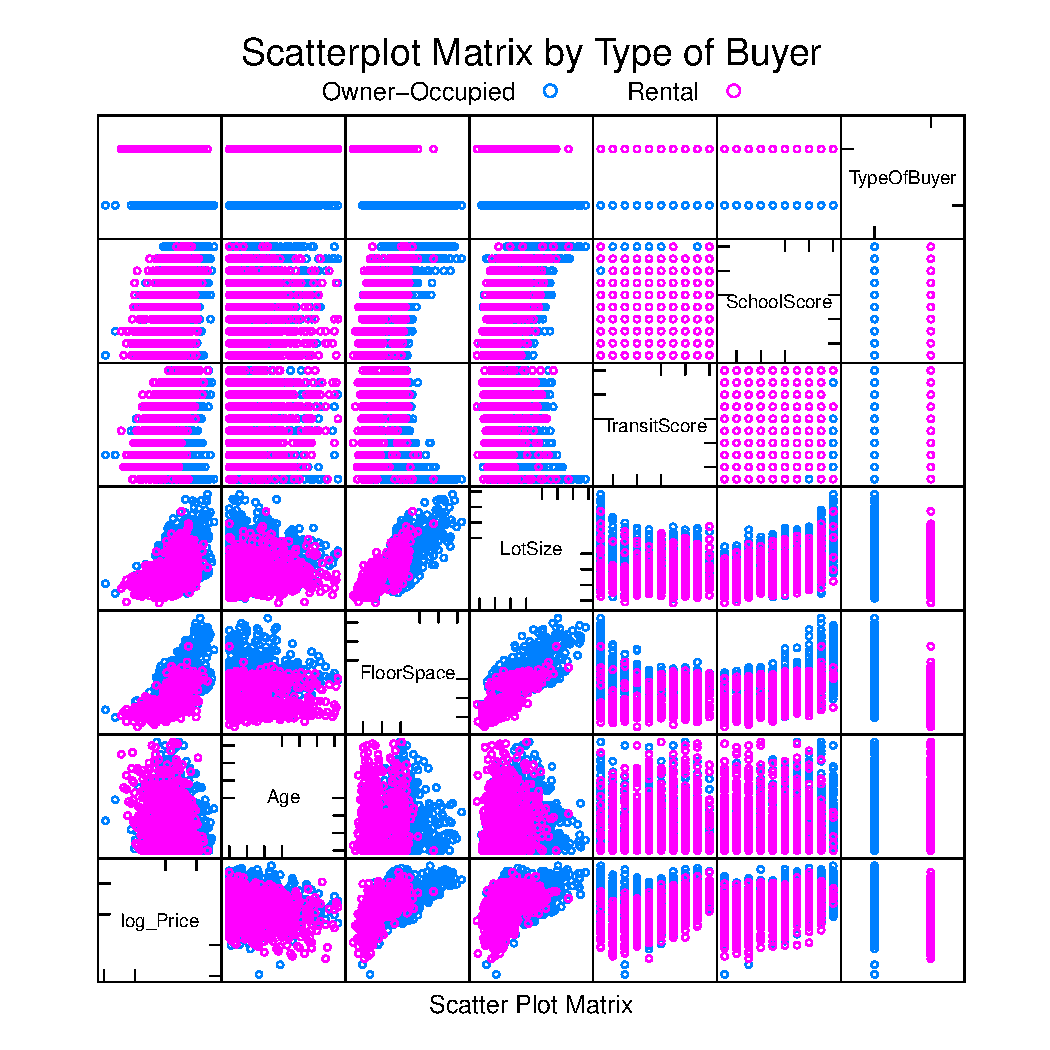
\includegraphics[scale = 0.5, keepaspectratio=true]{../Figures/slpom_by_buyer}
  \caption{Scatterplots with Categorical Variables Colored by Type of Buyer} \label{fig:slpom_by_buyer}
\end{figure}


\pagebreak

\subsection*{Spinograms by Type of Buyer}

Figure \ref{fig:buyer_and_EnclPatio_sales} depicts a spinogram
of the type of buyer and whether it has an enclosed patio.

\begin{figure}[h!]
  \centering
  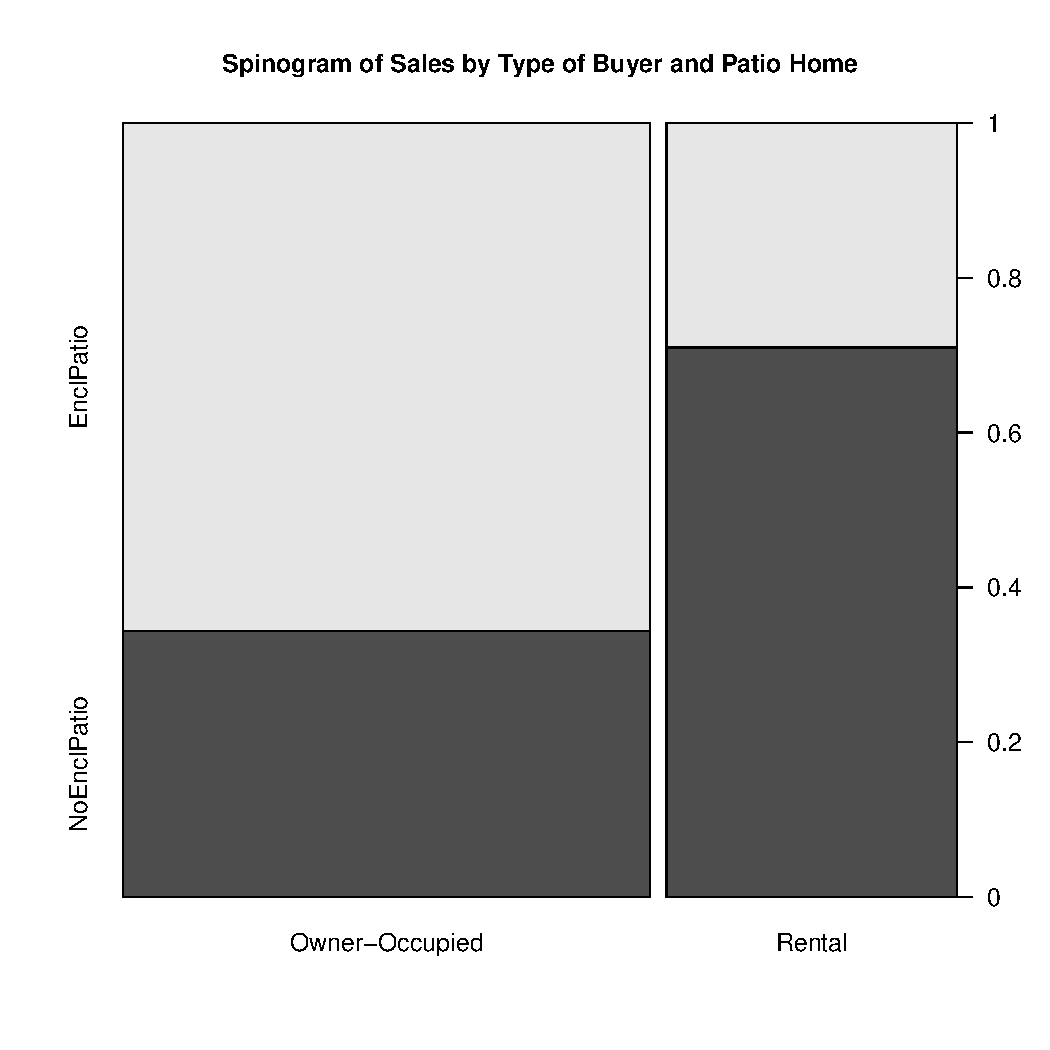
\includegraphics[scale = 0.5, keepaspectratio=true]{../Figures/buyer_and_EnclPatio_sales}
  \caption{Scatterplots by Type of Buyer and Patio} \label{fig:buyer_and_EnclPatio_sales}
\end{figure}

\pagebreak

Figure \ref{fig:buyer_and_SecGate_sales} depicts a spinogram
of the type of buyer and whether it has a security gate.

\begin{figure}[h!]
  \centering
  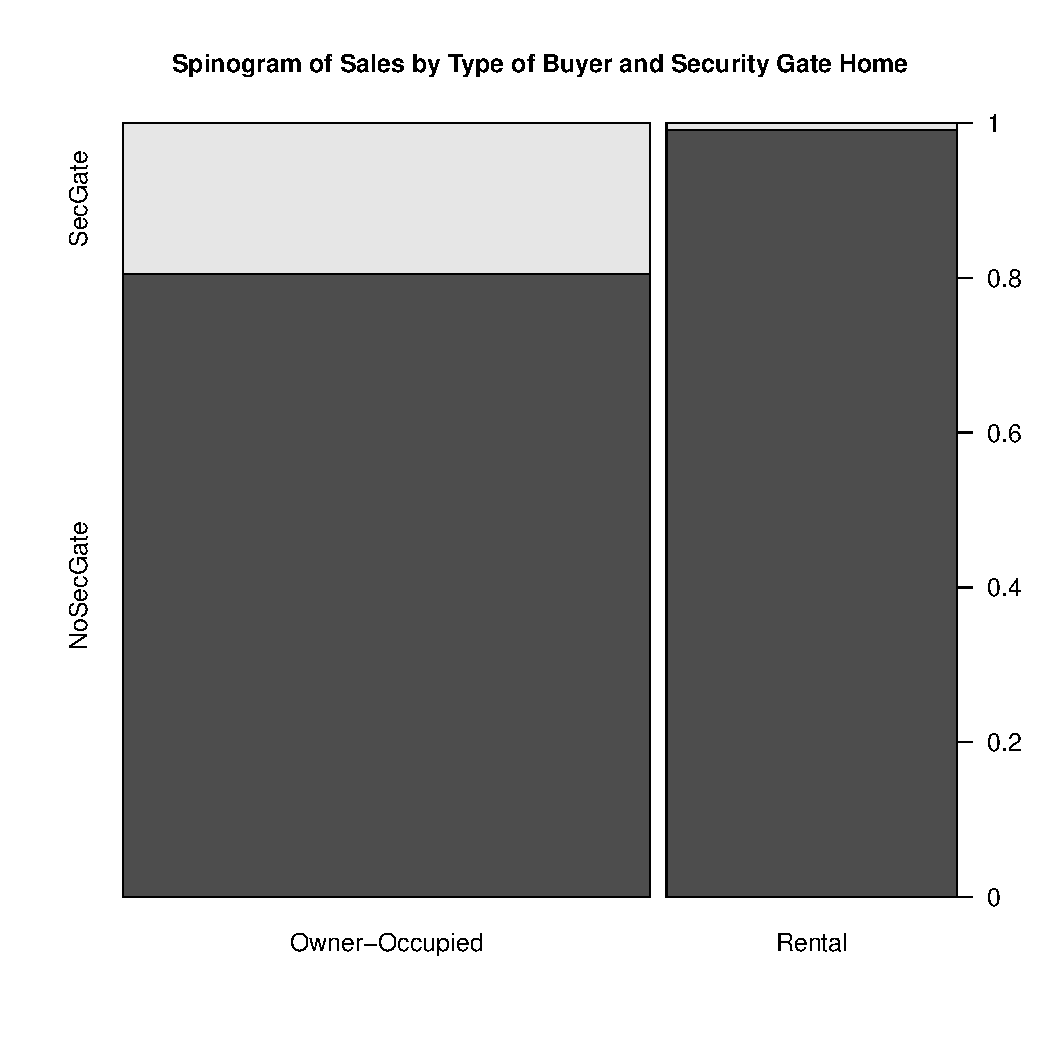
\includegraphics[scale = 0.5, keepaspectratio=true]{../Figures/buyer_and_SecGate_sales}
  \caption{Scatterplots by Type of Buyer and Securty Gate} \label{fig:buyer_and_SecGate_sales}
\end{figure}

\pagebreak

Figure \ref{fig:buyer_and_pool_sales} depicts a spinogram
of the type of buyer and whether it has an pool.

\begin{figure}[h!]
  \centering
  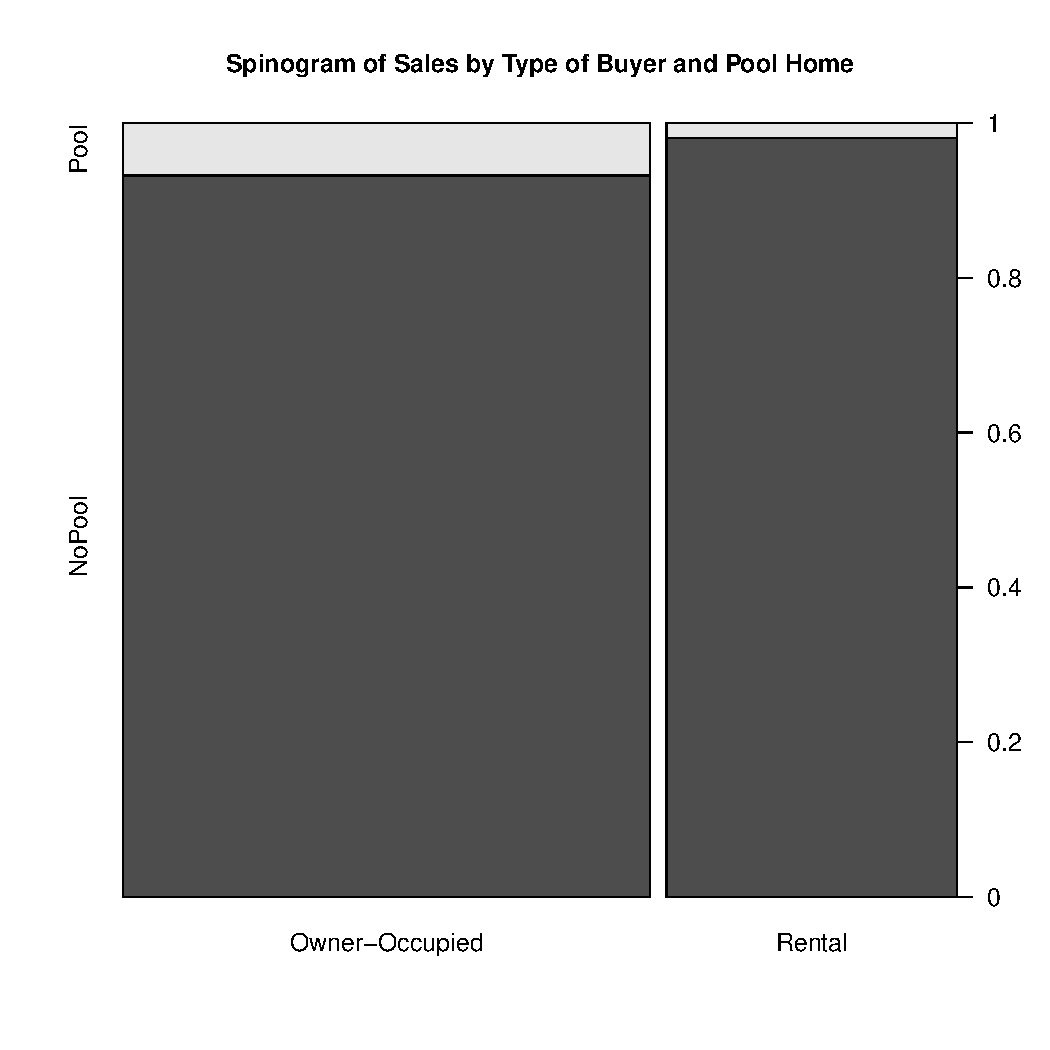
\includegraphics[scale = 0.5, keepaspectratio=true]{../Figures/buyer_and_pool_sales}
  \caption{Scatterplots by Type of Buyer and Pool} \label{fig:buyer_and_pool_sales}
\end{figure}

\pagebreak
\subsection*{Dot Chart byType of Buyer and Average Price}

Figure \ref{fig:dotchart_beds_TypeOfBuyer} depicts a dot chart
showing the average prices by number of bedrooms and type of buyer



\begin{figure}[h!]
  \centering
  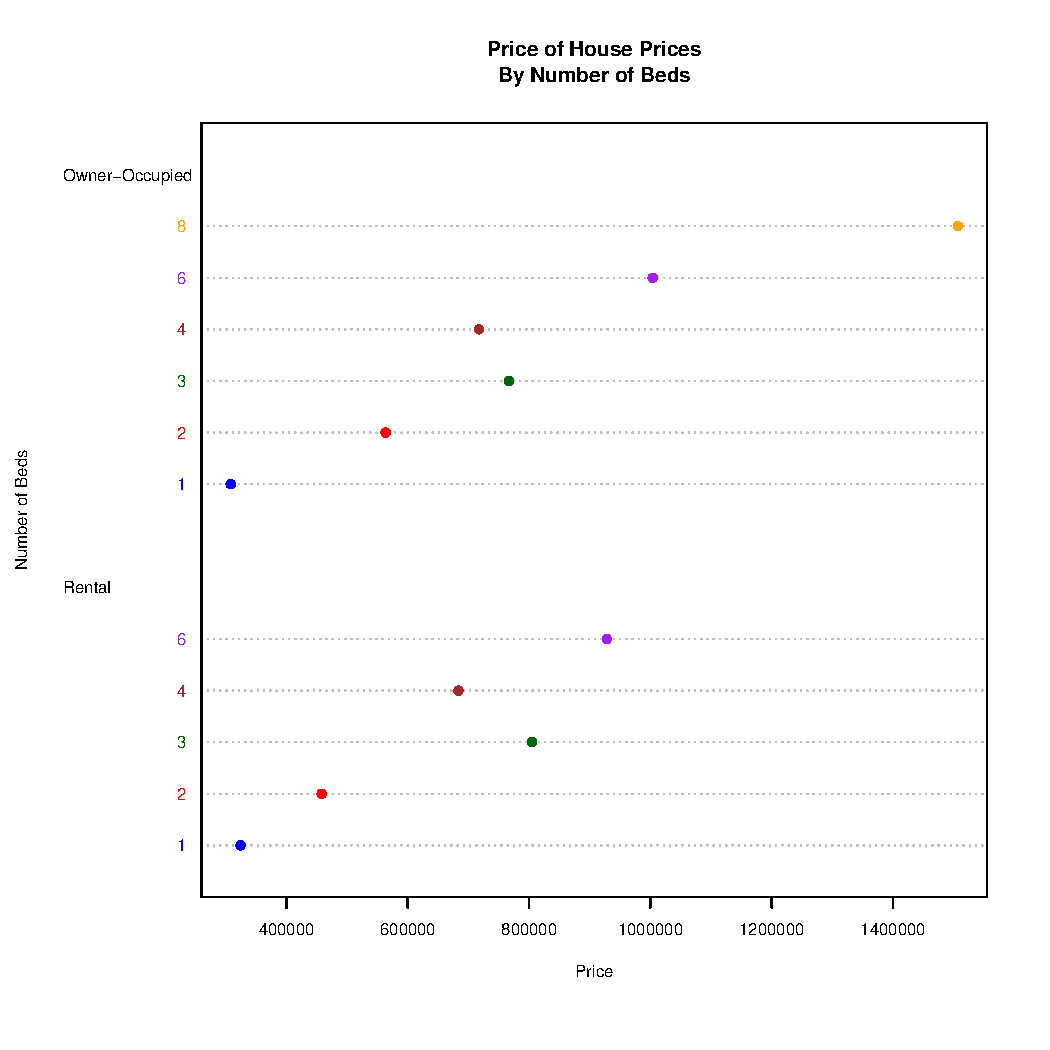
\includegraphics[scale = 0.5, keepaspectratio=true]{../Figures/dotchart_beds_TypeOfBuyer}
  \caption{Average Prices by Number of Bedrooms and Type of Buyer} \label{fig:dotchart_beds_TypeOfBuyer}
\end{figure}

\pagebreak
Figure \ref{fig:dotchart_baths_TypeOfBuyer} depicts a dot chart
showing the average prices by number of bedrooms and type of buyer


\begin{figure}[h!]
  \centering
  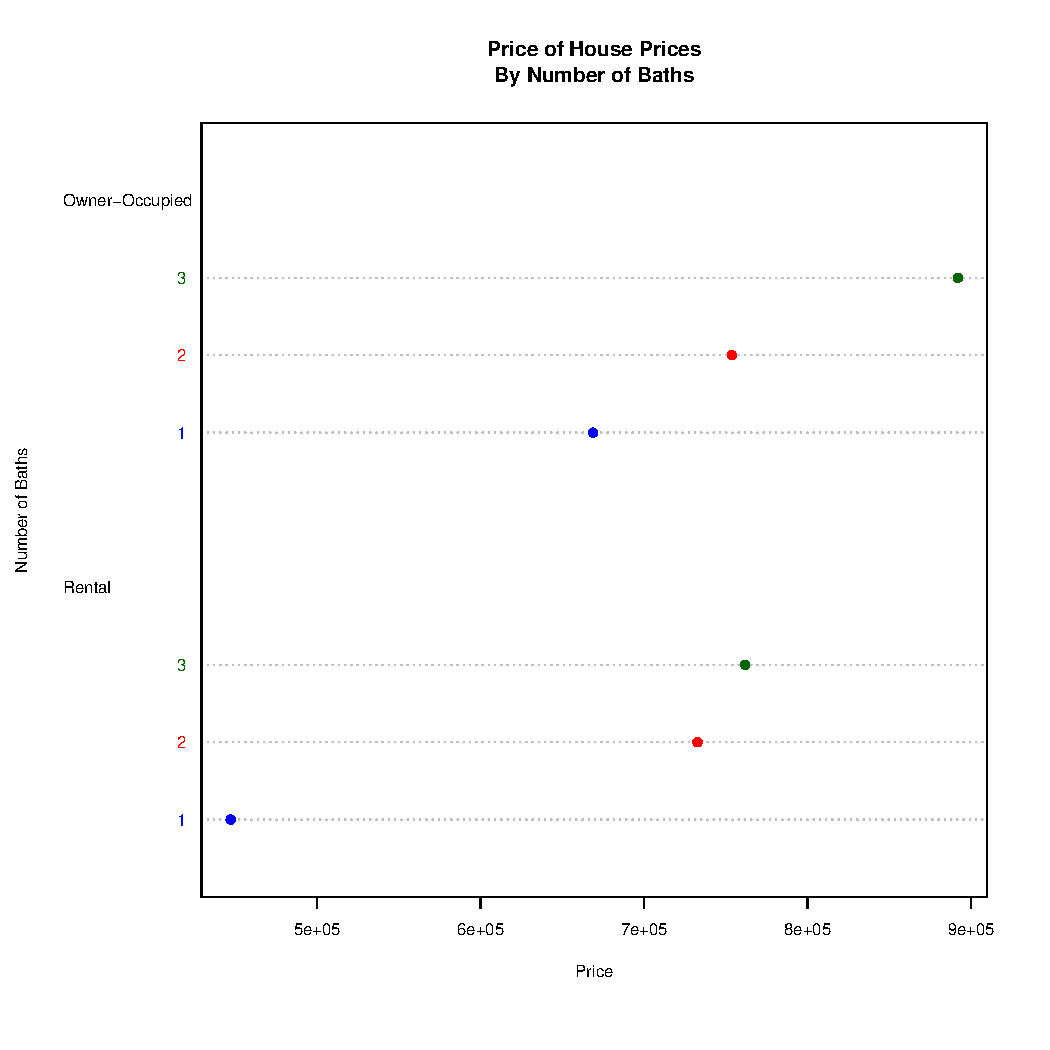
\includegraphics[scale = 0.5, keepaspectratio=true]{../Figures/dotchart_baths_TypeOfBuyer}
  \caption{Average Prices by Number of Bathrooms and Type of Buyer} \label{fig:dotchart_baths_TypeOfBuyer}
\end{figure}

\pagebreak
\subsection*{Summary}
Looking at the dot charts for number of bedrooms, we see that as the number of bedrooms increase,
the average price increases for both owner occupied and rental houses with the exception of 3 and 4 bedrooms where 
4 bedrooms average price is lower than 3 bedrooms. We also see that as the number of bathrooms increase, so does the average price
for both types of buyers. 1 bathroom rentals seem significantly cheaper than 1 bathroom owner occupied. The number of beds and nunber of baths 
is something I would like to keep in the regression model. Additionally, looking at whether it has a garage or not is also seems like a good variable to keep in the model.
Having a patio and secuirty gates may be two variables that need to be looked at more to see if they are suitable to be in the model. 


%%%%%%%%%%%%%%%%%%%%%%%%%%%%%%%%%%%%%%%%
%\end{document}
%%%%%%%%%%%%%%%%%%%%%%%%%%%%%%%%%%%%%%%%
